%% V1.0
%% by Gabriel Garcia, gabrcg@gmail.com
%% This is a template for Udacity projects using IEEEtran.cls

%% Be Udacious!

\documentclass[10pt,journal,compsoc]{IEEEtran}

\usepackage[pdftex]{graphicx}    
\usepackage{cite}
\hyphenation{op-tical net-works semi-conduc-tor}


\begin{document}

\title{Project Title}

\author{Author Name}

\markboth{Inference project, Robotic Nanodegree, Udacity}%
{}
\IEEEtitleabstractindextext{%

\begin{abstract}
Give an high level overview of work and results.
\end{abstract}

% Note that keywords are not normally used for peerreview papers.
\begin{IEEEkeywords}
Robot, IEEEtran, Udacity, \LaTeX, deep learning.
\end{IEEEkeywords}}


\maketitle
\IEEEdisplaynontitleabstractindextext
\IEEEpeerreviewmaketitle
\section{Introduction}
\label{sec:introduction}

\IEEEPARstart{H}{ere} you should explain your idea, introduce your robotic system, point some related works.

%example for inserting image
\begin{figure}[thpb]
      \centering
      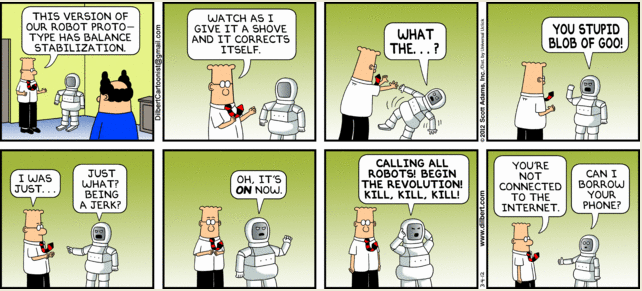
\includegraphics[width=\linewidth]{RobotRevolution5}
      \caption{Robot Revolution.}
      \label{fig:robot1}
\end{figure}

\subsection{Subsection Heading Here}
Subsection text here.

\subsubsection{Subsubsection Heading Here}
Subsubsection text here.


\begin{table}[h]
\caption{Table}
\label{table_example}
\begin{center}
\begin{tabular}{|c||c|}
\hline
One & Two\\
\hline
Three & Four\\
\hline
\end{tabular}
\end{center}
\end{table}



   

\section{Background}
Explain why you chose the network you did for the supplied data set and then why you chose the network used for your robotic inference project. \cite{lamport1994latex}

%example for Bullet point list

\begin{itemize}
\item example
\end {itemize}



%example for numbered list
\begin{enumerate}
\item example

\end{enumerate}

\section{Data Acquisition}
Why did you choose the data your did for your robotic inference project? How did you collect the data? What are important characteristics to capture in the data?

\section{Results}
Discuss the results of your trained robotics inference model and the model you used for the supplied data with the appropriate accuracy and inference time.

\section{Discussion}
Reflect on which is more important, inference time or accuracy, in regards to your robotic inference project.

\section{Future work}
How will you or did you leverage embedded workflow for personal growth in robotics? Would this be a commercially feasible product? Why or why not?

\bibliography{bib}
\bibliographystyle{ieeetr}

\end{document}